\documentclass[10pt]{article}

% Default 
\usepackage{graphicx}
\usepackage[
  backend=biber,
  style=numeric, 
  sorting=none
]{biblatex}

% Additional
\usepackage{amsmath}
\usepackage{textcomp}
\usepackage{gensymb}
\usepackage{placeins}
\usepackage{tabularray} 
\usepackage{xcolor}
\usepackage{placeins}
\usepackage{csquotes} 
\usepackage{todonotes}
\usepackage{hyperref}
\usepackage{siunitx}

\newcommand{\td}[1]{\todo[linecolor=blue, backgroundcolor=blue!25,bordercolor=blue, size=\small, inline]{#1}}

\addbibresource{references.bib}

\title{Diffraction and Interference} 
\author{Rahmanyaz Annyyev, Hikmat Gulaliyev}
\date{23 May, 2024} 

\begin{document}

\maketitle

\begin{abstract}

\td{Please expand more on the abstract to hit 200 words and include the information from the data calculation and discussion sections that you will write.}

The primary goal of this experiment is to examine the interference and diffraction phenomena when light passes through disparate apertures. The experiment is divided into two parts: part A and part B. In part A, the wavelength of the laser light is computed using a single-slit disk. In part B, the wavelength of the laser light is computed using a double-slit disk. The results of the experiment are presented in the tables below. The errors in the measurements are also calculated. The experiment makes several approximations, including the Fraunhofer diffraction pattern and coherent light. The discrepancies between the theoretical and experimental values are discussed. The experiment is concluded by summarizing the results and discussing the possible sources of error.

\end{abstract}

\section{Introduction}

\subsection*{General}

History bears witness to the fact that the nature of light has been a subject of debate for centuries. The wave theory of light, which posits that light is a wave, was first proposed by Christiaan Huygens in the 17th century. This theory was later supported by Thomas Young's double-slit experiment in the early 19th century. The wave theory of light was further developed by James Clerk Maxwell in the 19th century, who showed that light is an electromagnetic wave. The wave theory of light has been confirmed by numerous experiments, including the diffraction and interference of light.

Interference is a phenomenon that occurs when two or more coherent waves overlap. Coherent waves are waves that have the same frequency, wavelength, and constant relative phase. When coherent waves overlap, they interfere constructively or destructively, creating a pattern of light and dark regions on a screen. This pattern is known as an interference pattern.

Diffraction is a phenomenon similar to interference that occurs when light passes through a small aperture with dimensions on the order of the wavelength of light. When light passes through a small aperture, it diffracts, that is, it bends and spreads out in all directions. This creates a pattern of light and dark regions on a screen. This pattern is known as a diffraction pattern.

Both interference and diffraction can be explained by the Huygens-Fresnel principle, which states that each point on a wavefront acts as a source of secondary spherical wavelets. The interference of these secondary wavelets produces the diffraction and interference patterns observed in experiments.

The relative distances between the light source, the aperture, and the screen determine whether the diffraction pattern is in the near field or the far field. In the near field, the diffraction pattern is complex and varies with distance, and it is called the Fresnel diffraction pattern. In the far field, the diffraction pattern is simpler and does not vary with distance, since the secondary wavelets are approximately plane waves, and it is called the Fraunhofer diffraction pattern \cite{Hecht_2017}.

\subsubsection*{Single-Slit Diffraction}

The intensity of the light in the Fraunhofer diffraction pattern produced by a single slit is given by the equation
\begin{equation}
  I(\theta) = I_0 \left( \frac{\sin(\alpha)}{\alpha} \right)^2
  \label{eq:single-slit-intensity}
\end{equation}
where
\begin{equation}
  \alpha = \frac{\pi a \sin(\theta)}{\lambda}
\end{equation}
and $I_0$ is the intensity of the light at the center of the pattern, $a$ is the width of the slit, $\theta$ is the observation angle, and $\lambda$ is the wavelength of the light. The zeros of the diffraction pattern occur at those angles where $\sin(\alpha) = 0$, that is, at
\begin{equation}
  \sin(\theta) = \frac{n \lambda}{a} \quad \text{for} \quad n = \pm 1, \pm 2, \pm 3, \ldots
\end{equation}
One of our assumptions is that the width of the slit is much smaller than the distance from the slit to the screen, that is, $a \ll L$. In this case, $\sin(\theta) \approx \tan(\theta) = y/L$, where $y$ is the distance from the center of the pattern to the $n$th minimum. Therefore, the wavelength of the light can be computed using the equation
\begin{equation}
  \lambda = \frac{a \bar{y}}{L}
\end{equation}
where $\bar{y}$ is the average distance between adjacent minima. 

\subsubsection*{Double-Slit Interference}

The intensity of the light in the Fraunhofer diffraction pattern produced by a double slit when ignoring the effect of the slits is given by the equation
\begin{equation}
  I(\theta) = 4 I_0 \cos^2(\beta)
  \label{eq:double-slit-intensity-1}
\end{equation}
where
\begin{equation}
  \beta = \frac{\pi d \sin(\theta)}{\lambda}
\end{equation}
and $d$ is the distance between the slits, $\theta$ is the observation angle, and $\lambda$ is the wavelength of the light. It is assumed that the intensity produced by each slit is the same, that is, $I_1 = I_2 = I_0$. However, the intensity from a single-slit diffraction depends on the angle of observation. If we combine Equations \eqref{eq:single-slit-intensity} and \eqref{eq:double-slit-intensity-1}, we obtain the intensity of the light in the Fraunhofer diffraction pattern produced by a double slit as
\begin{equation}
  I(\theta) = I_0 \left( \frac{\sin(\alpha)}{\alpha} \right)^2 \cos^2(\beta)
  \label{eq:double-slit-intensity-2}
\end{equation}
The interference minima occur when
\begin{equation}
  \beta = (m + 1/2) \pi \quad \text{for} \quad m = 0, 1, 2, 3, \ldots
\end{equation}
and the maxima occur when
\begin{equation}
  \alpha = m \pi \quad \text{for} \quad m = 0, 1, 2, 3, \ldots
\end{equation}  
We will once again assume that the width of the slits is much smaller than the distance from the slits to the screen, that is, $d \ll L$. In this case, $\sin(\theta) \approx \tan(\theta) = y/L$, where $y$ is the distance from the center of the pattern to the $m$th minimum. Therefore, the wavelength of the light can be computed using the equation
\begin{equation}
  \lambda = \frac{d \bar{y}'}{L}
\end{equation}
where $\bar{y}'$ is the average distance between adjacent minima or maxima \cite{Pedrotti_2006}.

\subsection*{Procedure} 

The experiment is comprised of two parts: part A and part B. The setup consists of a diode laser with an output of $\lambda = 650 \pm 10\,\unit{nm}$, a light sensor, a linear translator, single and double-slit disks, a rotary motion sensor, an aperture bracket, and a PASCO{\textsuperscript\textregistered} data logger. As a preliminary step, we will spend some time to familiarize ourselves with various diffraction patterns caused by different slit widths and combinations of near and far field regions. The setup is shown in Figure (\ref{fig:1}).

\begin{figure}[ht]
  \centering
  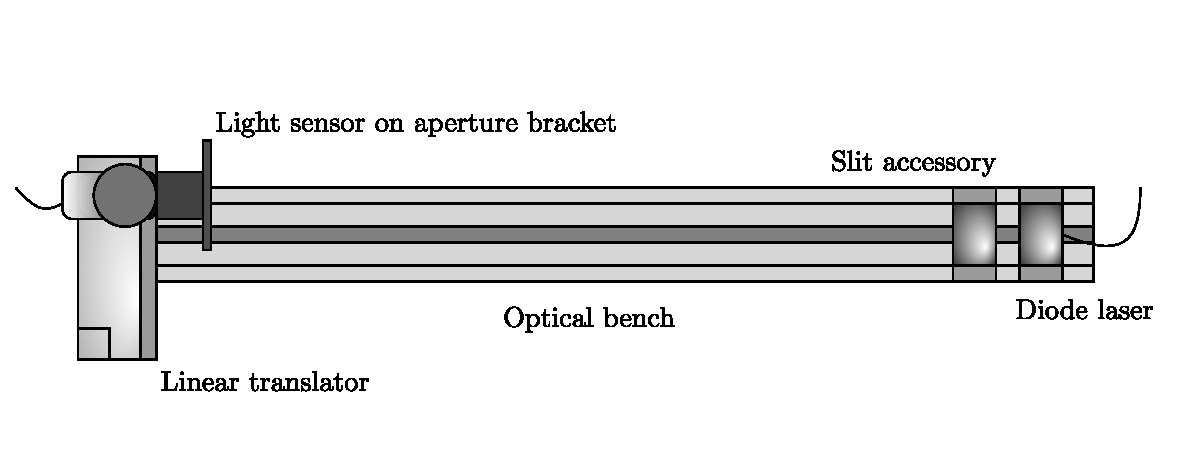
\includegraphics[scale=0.6]{figures/f1.pdf}
  \caption{The experimemtal setup.}
  \label{fig:1}
\end{figure}

\subsubsection*{Part A}

The purpose of part A is to compute the wavelength of the laser light using a single-slit disk.

First, we set up the components for the Fraunhofer diffraction pattern. The light sensor is placed on the aperture bracket, which is then mounted on the linear translator. The rotary motion sensor is attached to the linear translator. The single-slit disk is placed in front of the laser; both are placed at a certain distance from the light sensor. The whole setup rests on an optical bench.

Next, the laser is turned on, and the disk is rotated until the slit pattern is in line with the beam of the laser. If necessary, the adjustment screws on the back of the laser may be used to align the beam with the slit. 

Then, the pulley on top of the rotary motion sensor is rotated to move the sensor along the linear translator until a diffraction pattern appears on the white screen attached to the aperture bracket. 

After the pattern is visible, we have to ensure that it is horizontal and centered on the screen. The screws on the slit accessory can be used to obtain the desired pattern, and the accessory may be rotated to adjust the pattern's orientation.

Next, the aperture disk attached in front of the bracket is rotated to block ambient light and to ensure that the sensor is between maxima of the diffraction pattern. For the best results, the narrowest slit should be used.

Then, the light sensor is moved along the linear translator to align the center of the diffraction pattern with the slit on the aperture disk. The height of the sensor may be adjusted using the rod clamp on the rotary motion sensor.

Thereafter, the PASCO{\textsuperscript\textregistered} data logger is used to record the intensity of the light at different positions along the linear translator. The vertical axis of the graph should be set to the intensity of the light (light sensor output), and the horizontal axis should be set to the position of the sensor (rotary motion sensor output).

The procedure is repeated for different slit widths, and the data is recorded for each slit width in the corresponding table.

\subsubsection*{Part B}

The purpose of part B is to compute the wavelength of the laser light using a double-slit disk. The procedure is the same as in part A.

\section{Data \& Results}

The average distance between minima is calculated using the formula 
\begin{equation}
  \bar{y} = \frac{\lambda L}{a}
\end{equation}
where $\lambda$ is the wavelength of the light produced by the diode laser and is equal to \SI{650}{nm}.

\subsection*{Part A}

The results of part A are presented in Table (\ref{tab:1}).
\begin{table}[ht]
  \centering
  \begin{tblr}{
    cells = {halign = c, valign = m},
    column{1} = {halign = l},
    row{odd} = {bg = lightgray!5},
    hlines = {},
    vlines = {}
  }
    Pattern & A & B & C \\
    \hline 
    Width of the slit, $a$ (\si{\mm}) & 0.16 & 0.08 & 0.04 \\
    Distance from the slit to the screen, $L$ (\si{cm}) & 84.5 & 84.5 & 84.5 \\
    Average distance between minima, $\bar{y}$ (\si{cm}) & 0.34 & 0.69 & 1.37 \\
    $\bar{\lambda} = a\bar{y}/L$ (\si{nm}) & 644 & 653 & 649 \\
    Error $\Delta y$ in $\bar{y} = \sqrt{\sum_{i=1}^N (y_i - \bar{y})^2/(N-1)}$ (\si{cm}) \\
    Error $\Delta \lambda$ in $\bar{\lambda} = a \Delta y / L$ (\si{nm}) \\
    $\lambda = \bar{\lambda} \pm \Delta \lambda$ (\si{nm}) \\
  \end{tblr}
  \caption{Results of the first part of the experiment.}
  \label{tab:1}
\end{table}

\subsection*{Part B}

The results of part B are presented in Table (\ref{tab:2}).

\begin{table}[ht]
  \centering
  \begin{tblr}{
    cells = {halign = c, valign = m},
    column{1} = {halign = l},
    row{odd} = {bg = lightgray!5},
    hlines = {},
    vlines = {}
  }
    Pattern & D & E & F \\
    \hline 
    Width of the slit, $d$ (\si{\mm}) & 0.5 & 0.25 & 0.125 \\
    Distance from the slit to the screen, $L$ (\si{cm}) & 84.5 & 84.5 & 84.5 \\
    Average distance between minima, $\bar{y}$ (\si{cm}) & 0.11 & 0.22 & 0.44 \\
    $\bar{\lambda} = d\bar{y}/L$ (\si{nm}) & 651 & 651 & 651 \\
    Error $\Delta y$ in $\bar{y} = \sqrt{\sum_{i=1}^N (y_i - \bar{y})^2/(N-1)}$ (\si{cm}) \\
    Error $\Delta \lambda$ in $\bar{\lambda} = d \Delta y / L$ (\si{nm}) \\
    $\lambda = \bar{\lambda} \pm \Delta \lambda$ (\si{nm}) \\
  \end{tblr}
  \caption{Results of the second part of the experiment.}
  \label{tab:2}
\end{table}

\section{Discussion \& Conclusion}

\subsection*{Errors}

\subsection*{Approximations}

The experiment makes several approximations. Some of them are as follows:

\begin{itemize}
  \item \textbf{Fraunhofer diffraction pattern:} The experiment assumes that the diffraction pattern is in the far field, that is, the distance from the slit to the screen is much larger than the width of the slit. This assumption is necessary to simplify the calculations and to obtain a simpler diffraction pattern. 
  \item \textbf{Coherent light:} The experiment assumes that the light from the laser is coherent, that is, the light waves have the same frequency, wavelength, and constant relative phase. In reality, the light from the laser may not be perfectly coherent, which may affect the diffraction pattern.
\end{itemize}

\subsection*{Discrepancies}

\subsection*{Conclusion} 

\section{Extra Credit}

One of the applications of diffraction is in the field of X-ray crystallography. It is a domain of experimental science concerned with the arrangement of atoms and molecules in a crystal. The underlying principle of X-ray crystallography is that the atoms in a crystal scatter X-rays in different directions, creating a diffraction pattern. By analyzing the diffraction pattern, scientists can determine the structure and properties of the crystal. X-ray crystallography has numerous applications in chemistry, biology, and materials science, including drug design, protein structure determination, and material characterization \cite{Carvalho_2009}.

Before the discovery of X-ray diffraction, the structure of the crystals was determined by primitive methods. The X-rays were discovered by Wilhelm Conrad Röntgen in 1895, and x-ray diffraction was discovered by Max von Laue in 1912. He bombarded crystals with X-rays in hopes of determining the nature of X-rays. The diffraction pattern confirmed the wave nature of X-rays and the periodic arrangement of atoms in crystals. The diffraction pattern was later analyzed by William Henry Bragg and his son William Lawrence Bragg, who developed Bragg's law in 1912--1913, which relates the angle of diffraction to the spacing of the atomic planes in the crystal. The Bragg's law is given by the equation
\begin{equation}
  n \lambda = 2 d \sin(\theta)
\end{equation}
where $n$ is an integer, $\lambda$ is the wavelength of the x-rays, $d$ is the spacing of the atomic planes, and $\theta$ is the angle of diffraction. By measuring the angle of diffraction and the wavelength of the x-rays, scientists can determine the spacing of the atomic planes in the crystal. The Braggs were awarded the Nobel Prize in Physics in 1915 for their work on X-ray crystallography \cite{Bragg_1913}.

In biology, molecules are often too small to be seen with a light microscope. X-ray crystallography allows scientists to determine the structure of these molecules at the atomic level. This has led to numerous discoveries in biology, including the solution of cholesterol (1937), penicillin (1945), vitamin B\textsubscript{12} (1956) by English chemist Dorothy Crowfoot Hodgkin, for which she was awarded the Nobel Prize in Chemistry in 1964. The three-dimensional structure of penicillin is shown in Figure (\ref{fig:2}).

\begin{figure}[ht]
  \centering
  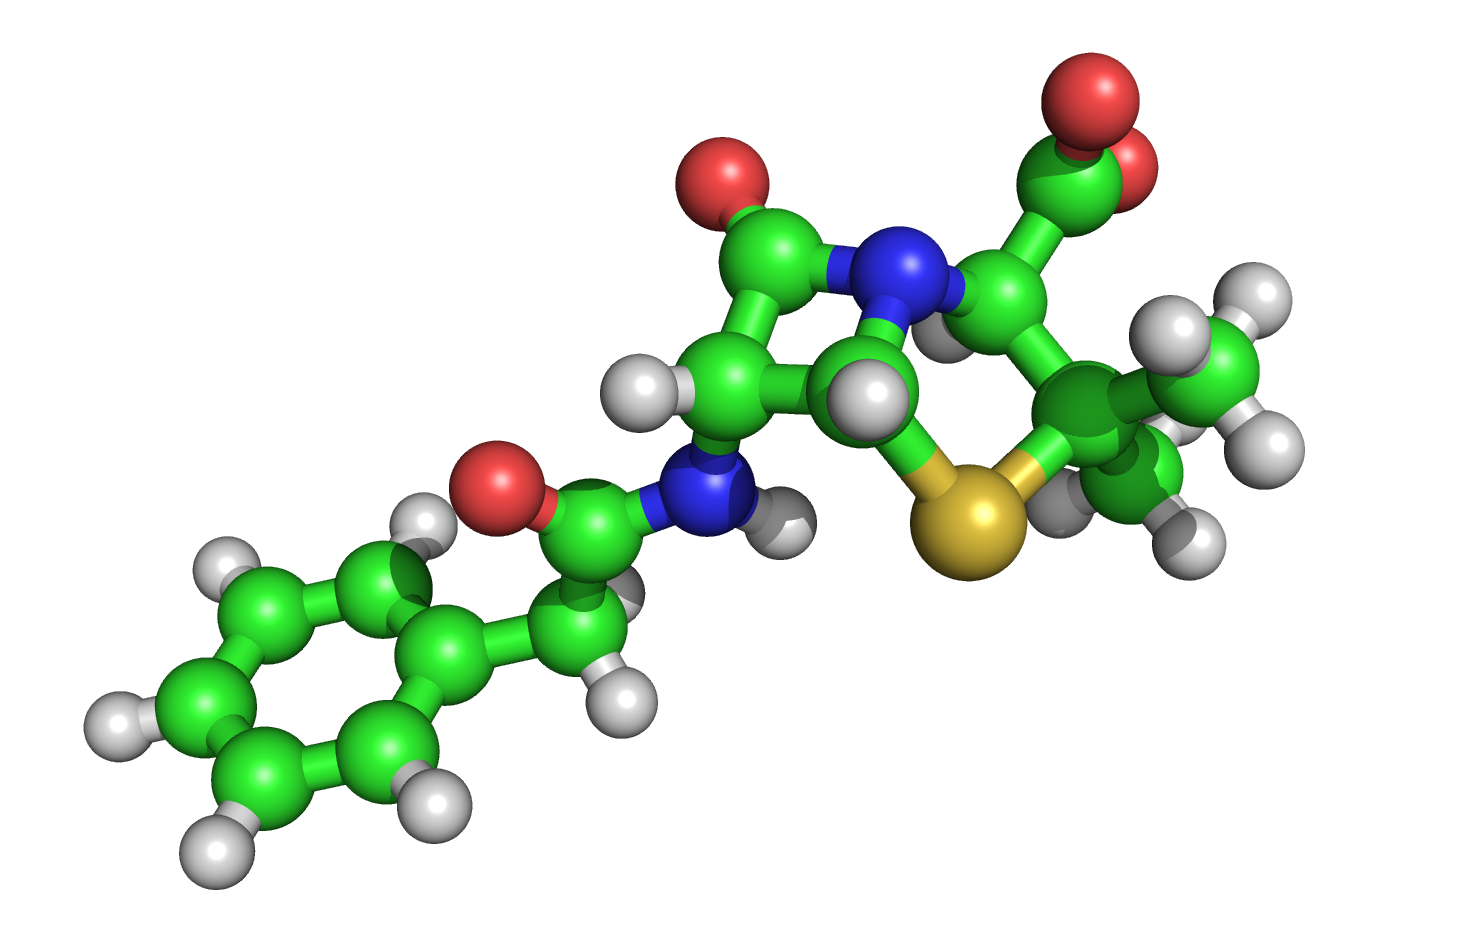
\includegraphics[scale=0.2]{figures/f2.png}
  \caption{The three-dimensional structure of penicillin. Image credit: Bassophile (Creator). July 12, 2007. Retrieved May 26, 2024, from: \url{https://commons.wikimedia.org/w/index.php?curid=17230435}}
  \label{fig:2}
\end{figure}

One of the important applications of X-ray crystallography is in drug discovery and design. By determining the structure of a protein or enzyme, scientists can design drugs that target the protein or enzyme and inhibit its activity. This has led to the development of numerous drugs, including antibiotics, antiviral drugs, and anticancer drugs. X-ray crystallography has also been used to determine the structure of DNA, which has revolutionized the field of genetics and molecular biology. The discovery of the double helix structure of DNA by James Watson and Francis Crick in 1953 was based on x-ray diffraction data obtained by Rosalind Franklin and Maurice Wilkins. X-ray crystallography has also been used to determine the structure of many other biological molecules, including proteins, nucleic acids, and carbohydrates \cite{Bijak_2023}.

\printbibliography

\end{document}